\documentclass[11 pt]{article}
\usepackage[left=0.95in,top=0.9in,bottom=0.9in,right=0.95in,nohead,nofoot]{geometry}
\usepackage[hidelinks]{hyperref}  % get rid of boxes around links 
\usepackage[usenames]{color}
\hypersetup{colorlinks=true,citecolor=black,urlcolor=blue}
\usepackage[left,running]{lineno}
% \linenumbers
\renewcommand*{\thefootnote}{\fnsymbol{footnote}}
\makeatletter
\renewcommand{\@makefnmark}{\hbox{\textsuperscript{\normalsize{\@thefnmark}}}}
\makeatother
\usepackage{graphicx, fullpage}
% \usepackage[parfill]{parskip}
\usepackage{float}
\usepackage{color}

\begin{document}
\pagestyle{empty}

{\centering\section*{How Biases Scale in Landcover Data, With Implications for Area-based Estimates}}

\section*{Overview}
This paper explores the biases inherent in current landcover products' estimates of cropland cover, and the implications that these biases have for research making area-related inferences using these data (e.g. estimates of carbon stocks; crop production and yield; land use change studies). This analysis was made possible by the existence of a high accuracy, hand-digitized cropland data layer available for South Africa, which provides an objective and spatially extensive standard of ``truth'' against which landcover products can be assessed.  

\section*{Framing}
This paper has relevance for any field that makes use of landcover data, so I want to try target a high visibility journal. Nature would be nice, but that is a big ask, The problem is that an editor might look at this very quickly and say that is too specialized or local, so it has to have a pretty good sales pitch if we are to avoid having it go into a trade journal (e.g. \emph{Remote Sensing of Environment}). PloS One might be a good fit, given that it accepts papers across multiple disciplines provided they are technically sound. Thoughts (including ideas for a better title)?  

General approach/rationale: 

\begin{enumerate}
  \item Satellite-derived landcover data are a key ingredient for understanding many aspects of environmental, social, and economic change. Examples:
    \begin{itemize}
      \item Food production estimates (e.g. yield gaps) - anything by RamanFoley, Rachel's work, etc.
      \item Carbon stocks (Tier 1 vegetated carbon estimates) - Ruesch and Gibbs
      \item Habitat loss data.
      \item Attempts to estimate land-atmosphere interactions, hydrological models, etc. [Here we will run land surface model with GTI cropland fraction providing the cropland surface, and we will then alter this using the bias rasters to see how this propagates into ET and runoff estimation errors, etc] 
    \end{itemize}
  \item It is understood that there are errors inherent in these data, particularly global-scale products, and that there is great discrepancy between these. This is particularly true of developing regions that will experience the largest amount of land surface change this century, such as Africa.  
    \begin{itemize} 
      \item Cite to Fritz's papers (from geowiki). 
      \item Emphasize what they did so that we can differentiate--they look primarily at disagreements between products, and how much it affects country level estimates. Also focus on older generation datasets. 
    \end{itemize}
  \item What is less known is how much bias these landcover errors might introduce into research findings that depend on areas estimates drawn from landcover data. Such an assessment depends on having accurate, spatially extensive landcover data to assess large areas, which are typically not available. 
  \item In this study, we use a unique, high accuracy agricultural landcover dataset to assess the biases in the most current landcover datasets, looking at bias as a function of spatial scale and landcover fraction.  
  \item Our goal is to provide insight--for users of landcover products across a range of disciplines--into: 
    \begin{itemize}
      \item The scales at which area-based inferences drawn from global landcover products are appropriate
      \item How variations within landcover properties may influence bias
      \item Which datasets are most appropriate for making inferences
    \end{itemize}
\end{enumerate}

\section*{Key Results}
\begin{enumerate}
  \item Bias as a function of scale
    \begin{enumerate}
    \item At 1 km resolution all landcover products are still fairly biased.  Actual bias is lowest in the geowiki dataset (+5\% under-estimate, on average, Figure 2), followed by the higher resolution South Africa landcover (SALC) dataset (8\% over-estimate, Figure 2), but the absolute bias is much higher in geowiki (23\%, Figure 3) than the SA dataset 11\%). The other products (MODIS and GlobCover) are grossly biased at the 1 km resolution (21-34\% under-estimates; 31-35\% mean bias).
      \begin{itemize}
         \item This discrepancy between actual and absolute biases for the two datasets (geowiki \& SALC) reflect the spatial variability of biases--geowiki underestimates cropland fraction in the west and overestimate in the north and east, whereas SALC's biases are all of over-estimation. 
      \end{itemize}
    \item Bias drops to acceptable levels quickly for geowiki--at 5X5 km, mean bias is just 1\% (overestimated). The absolute bias for this dataset is 10\% or lower from 10X10 km resolution and coarser.  
    \item The SA dataset's bias is fairly consistent but low across all levels of aggregation, amounting to no more than an 8\% overestimate of cropland with absolute bias of similar magnitude. 
    \item MODIS and GlobCover biases (mostly of underestimation) do not dissipate until the higher levels of aggregation. MODIS's actual bias (under-estimation) falls below 10\% at 20 km resolution, but the absolute bias remains above 10\% until more than a 100-fold aggregation is done ($>$100 km resolution).  For GlobCover, it needs to be more than 200-fold.  
    \end{enumerate}
  \item Bias as a function of cropland cover
    \begin{enumerate}
      \item Biases are highest when pixels contain intermediate levels of cropland cover.  This is particularly evident in the distributions of absolute biases (Figure 3) at the finer spatial scales ($\leq$20 km). The highest biases are associated with cropland cover of 50-75\%.
       \begin{itemize} 
         \item Classification algorithms are thus more error-prone where landcover is mixed/heterogenous.
        \end{itemize}
      \item The exception to this lies in the GlobCover dataset, where bias primarily increases as a function of cropland cover. The reason for this is that GlobCover's cropland classes do not provide for 100\% cropland cover, so aggregation tends to exacerbate underestimates. 
      \begin{itemize} 
        \item An example illustrats this: take 4 1 km pixels, 2 of which are 100\% cropland, 2 of which are other cover types. Imagine a landcover product classifies 3 of these as cropland (2 correct, 1 an error of commission), using a cropland class that is defined as 50\% cropland. Aggregating the actual fraction by a factor of 4 will result in a new 4 km pixel having 50\% cropland, whereas aggregating the landcover product's pixels will give just 38\% cropland, even when factoring in the incorrect classification.)
        \end{itemize}
    \end{enumerate}
  \item Bias as a function of method
      \begin{enumerate}
      \item Higher resolution and ensemble-based approaches have less bias.
      \item geowiki represents a fusion of multiple coarse resolution data sources that has undergone extensive validation using a crowdsourcing approach
      \item the SALC dataset is based on 30 m landsat data, but incorporates a range of ancillary data and expert judgement
      \item MODIS and GlobCover data are effectively single source/single algorithm. 
    \end{enumerate}
\end{enumerate}

%\vspace{0.5 in}
\begin{figure}[H]
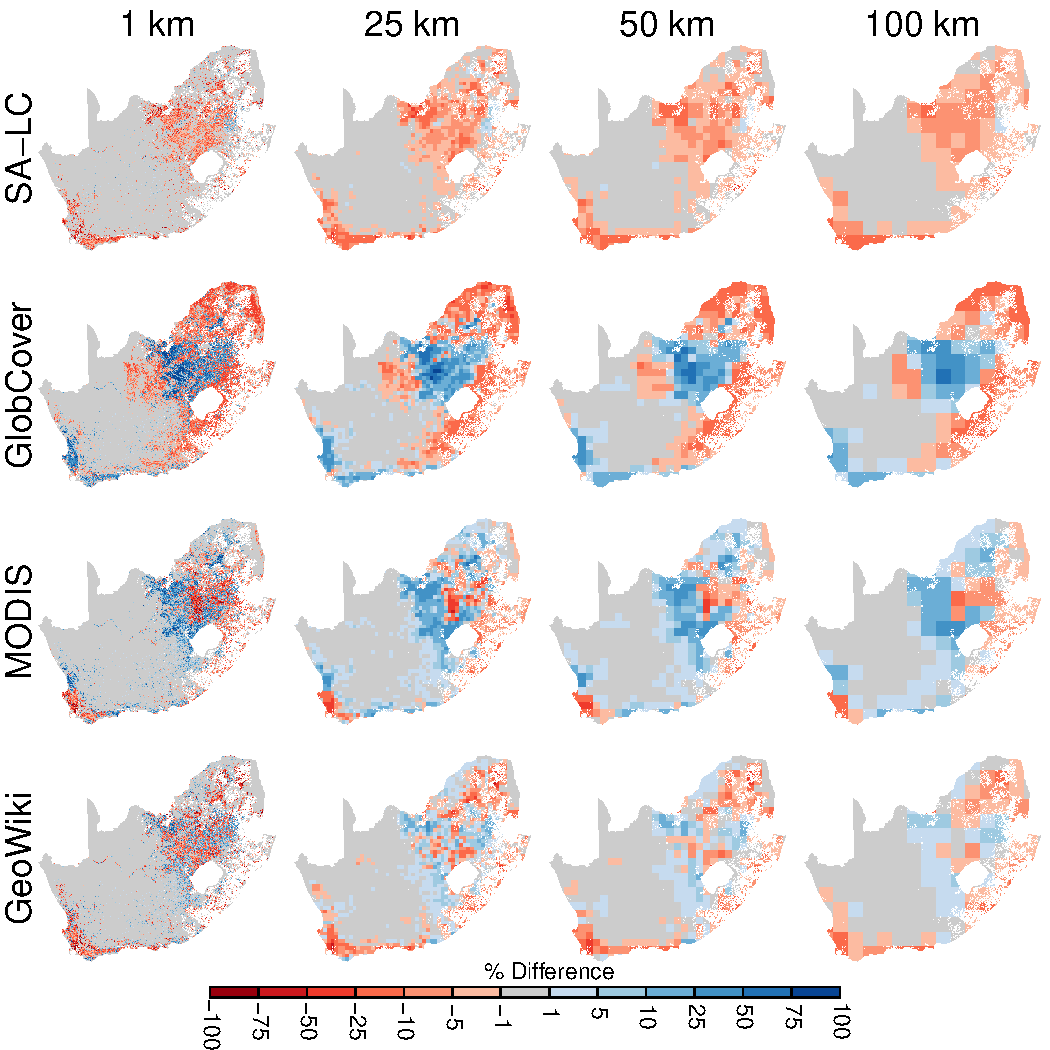
\includegraphics[width = \linewidth]{../figures/bias_map.pdf}
\caption{The spatial distribution of biases in cropland cover estimates from four landcover products, calculated by subtracting each of their cropland percentage estimates from that of GeoTerraImage's cropland data layer. The biases were calculated for several different levels of, ranging from the original 1 km resolution up to 300 km (only 1, 25, 50, and 100 km results are shown here). Blue areas are those where the landcover products underestimated croplands, and red areas are where they overestimated. The GlobCover and MODIS results are drawn from biases calculated from the intermediate cropland fraction estimates per pixel.}
\end{figure}
%\vspace{-0.3in}

\begin{figure}[H]
\begin{center}
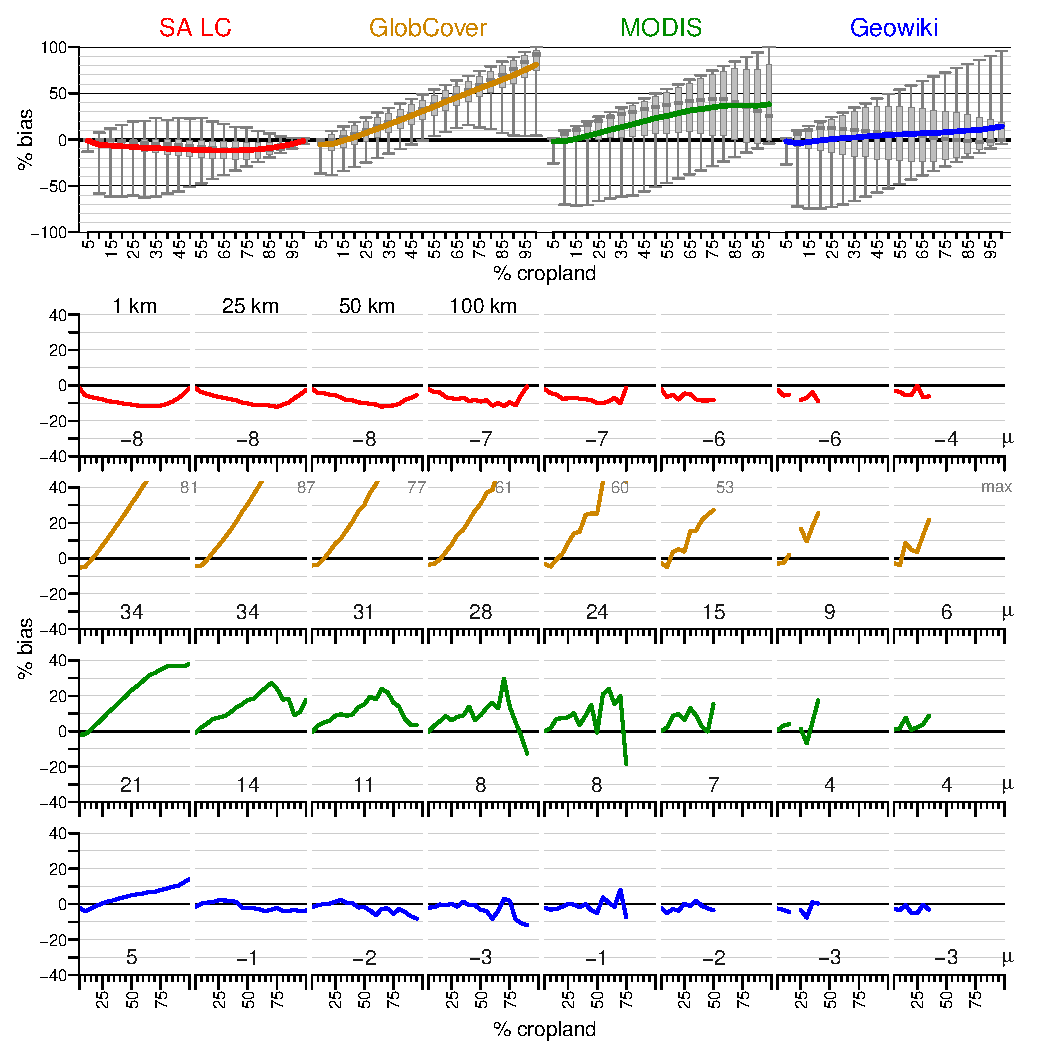
\includegraphics[width = \linewidth]{../figures/bias_act.pdf}
\caption{The statistical distribution of biases in cropland percentage estimates, in relation to different levels of cropland cover measured by the GeoTerraImage data (grouped into classes spanning 5\%). The top row shows biases at 1 km resolution for each of the four assessed landcover datasets, including the 2.5$^{th}$, 25$^{th}$, 50$^{th}$, 75$^{th}$, and 95$^{th}$ percentile values (grey box plots), as well as the means (colored lines). Rows 2-5 illustrate how mean biases for each landcover product (rows) changes in relation to the level of aggregation (columns). Mean biases greater than 40\% are truncated in order to improve plot clarity (the maximum truncated value is provided at the top right of each plot in grey). The mean bias across all cropland classes is provided at the bottom of each panel. Each 5\% cropland classes is represented by its upper bound on the X-axis (e.g. 5 for the 0-5\% class).}
\end{center}
\end{figure}

\begin{figure}[H]
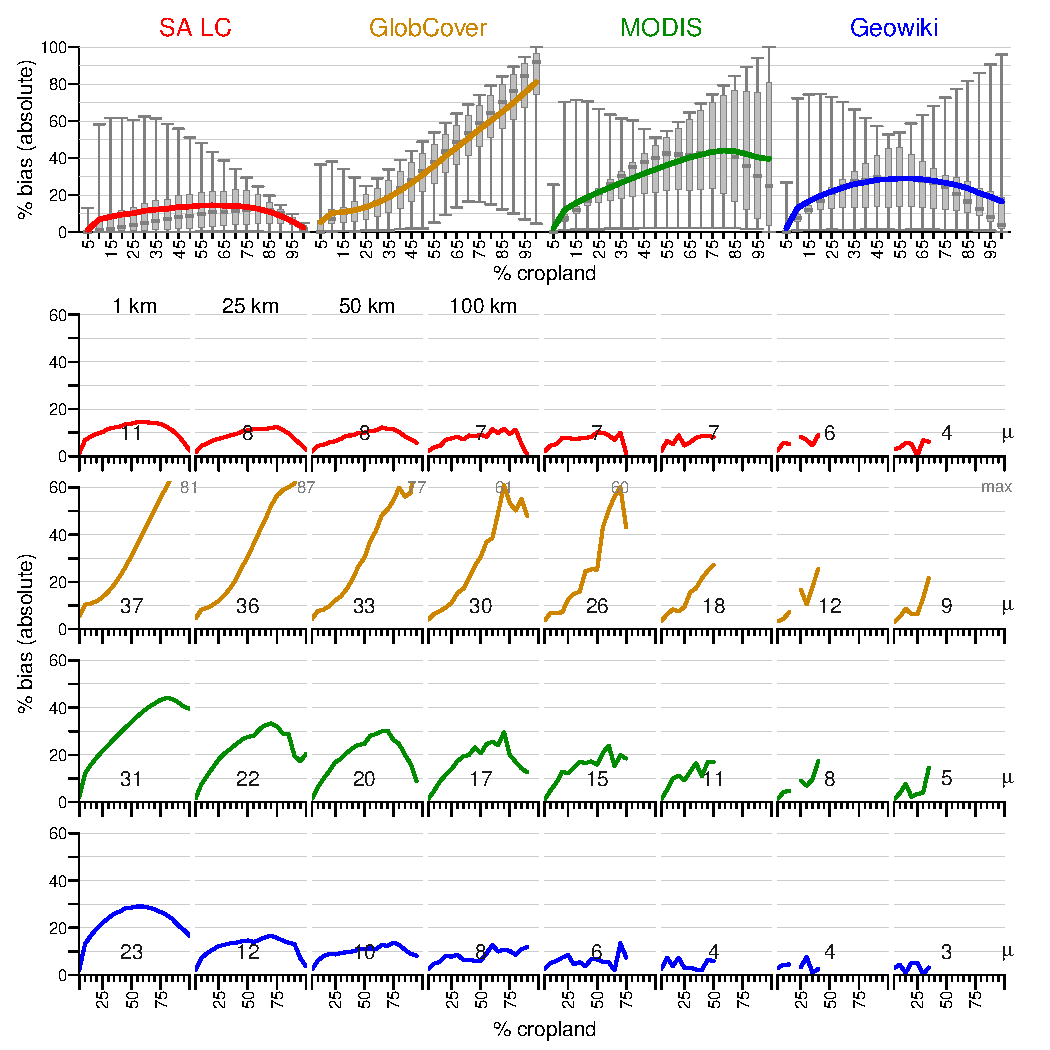
\includegraphics[width = \linewidth]{../figures/bias_abs.pdf}
\caption{The statistical distribution of \emph{absolute} biases in cropland percentage estimates, in relation to different levels of cropland cover measured by the GeoTerraImage data (grouped into classes spanning 5\%). The top row shows \emph{absolute} biases at 1 km resolution for each of the four assessed landcover datasets, including the 2.5$^{th}$, 25$^{th}$, 50$^{th}$, 75$^{th}$, and 95$^{th}$ percentile values (grey box plots), as well as the means (colored lines). Rows 2-5 illustrate how mean \emph{absolute} biases for each landcover product (rows) changes in relation to the level of aggregation (columns). Mean biases greater than 40\% are truncated in order to improve plot clarity (the maximum truncated value is provided at the top right of each plot in grey). The mean \emph{absolute} bias across all cropland classes is provided at the bottom of each panel. Each 5\% cropland classes is represented by its upper bound on the X-axis (e.g. 5 for the 0-5\% class).}
\end{figure}

\section*{Implications}
\begin{enumerate}
  \item At finer resolutions, only high resolution or newer, fusion-based landcover products are appropriate for making area-based inferences
    \begin{itemize}
      \item At 1-10 km resolution, high resolution products are least biased. Such products are typically not available globally, but new technologies (processing, high resolution imagery) are making it increasingly feasible to generate them (cite Hansen's forest product)
      \item The geowiki dataset has sufficiently low biases at resolutions of 20 km and coarser. It also demonstrates a methodological aspect that is evident in other fields (climate modeling, crop modeling, species distribution modeling)--ensemble based approaches return more accurate results than single method approaches.  
    \end{itemize}
  \item If you have to rely on single source datasets, e.g. for mapping landcover change, than substantial aggregation is necessary before area-based inferences can be made with confidence. Country-scales or higher should be appropriate. 
  \begin{itemize} 
    \item Illustrative examples: 
      \begin{itemize} 
        \item Examples from actual papers - Convergence of yield or carbon estimates at regional scale from our (Tim) savannas paper, emphasizing discrepancy between cropland fractions; discuss that Tier 1 carbon estimates from Gibbs et al use the GLC2000 dataset, the predecessor of GlobCover.  
         \item Maybe another example from the literature - habitat conversion, or crop yield estimates, or thinking about how a land surface model might be impacted (Justin?)
      \end{itemize}
    \item But care should be taken when aggregating--the characteristics of cropland in a country will influence this bias. 
      \begin{itemize}
        \item For example, if a high percentage of a region's cropland is of a mixed/mosaic type (e.g. fields interleaved with natural vegetation, such that $\sim$50\% is cropland), then aggregated biases may be higher.  
        \item This is the sort of situation that is more likely to occur in the smallholder dominated systems, which are dominant in many other African countries (where a high proportion of trees in fields may exacerbate classification errors). It is less likely in larger-scale commercial agriculture of the sort that dominates South Africa. 
        \item We could not test this aspect here, as we had to explicitly exclude smallholder/communal farmlands from our analysis because they were not mapped with the same precision, so the degree to which bias in this sort of cropland differs from commercial croplands requires further investigation \textbf{this sets up one aspect of the second paper, Stephanie}.  
      \end{itemize}
  \end{itemize}
  
\end{enumerate}

\section*{Methods}
\subsection*{Figures, tables, stats needed}
\begin{itemize}
  \item Distribution of accuracy assessment plots
  \item Close-up of polygons (maybe)
  \item Country level bias means/bar plot of means
\end{itemize}


\end{document}

